%!TEX root=paper.tex

\subsection{Performance}
\label{sec:perf}

% The \tool also collects information regarding endpoint performance. 
The \perspective{API Performance} visualization perspective presents
an overview of the response times for all the tracked endpoints 
by using a box-and-whiskers plot. 

\Fref{fig:ep} presents such a perspective from our case study which 
was taken in the last quarter of 2017. Several observations are 
straightforward: 

\begin{itemize}

  \item The slowest endpoint and the one with the highest variability is \epFeedItemsColor: it retrieves a list of recommended articles for a given user. Since a user can be subscribed to anything from one to three dozen article sources, and since the computation of the difficulty was done in real time, the variability in time among users is likely to be very large. 

  \item \epTranslationsColor and \epBookmarksToStudyColor, two of the most used endpoints (as seen in \Fref{fig:aeu}) are also some of the slowest and with most outliers. The first one is very critical for the usability of the Reader applications since it called when a user taps on a word to receive a translation.
 
\end{itemize}

\begin{figure}
 \centering
 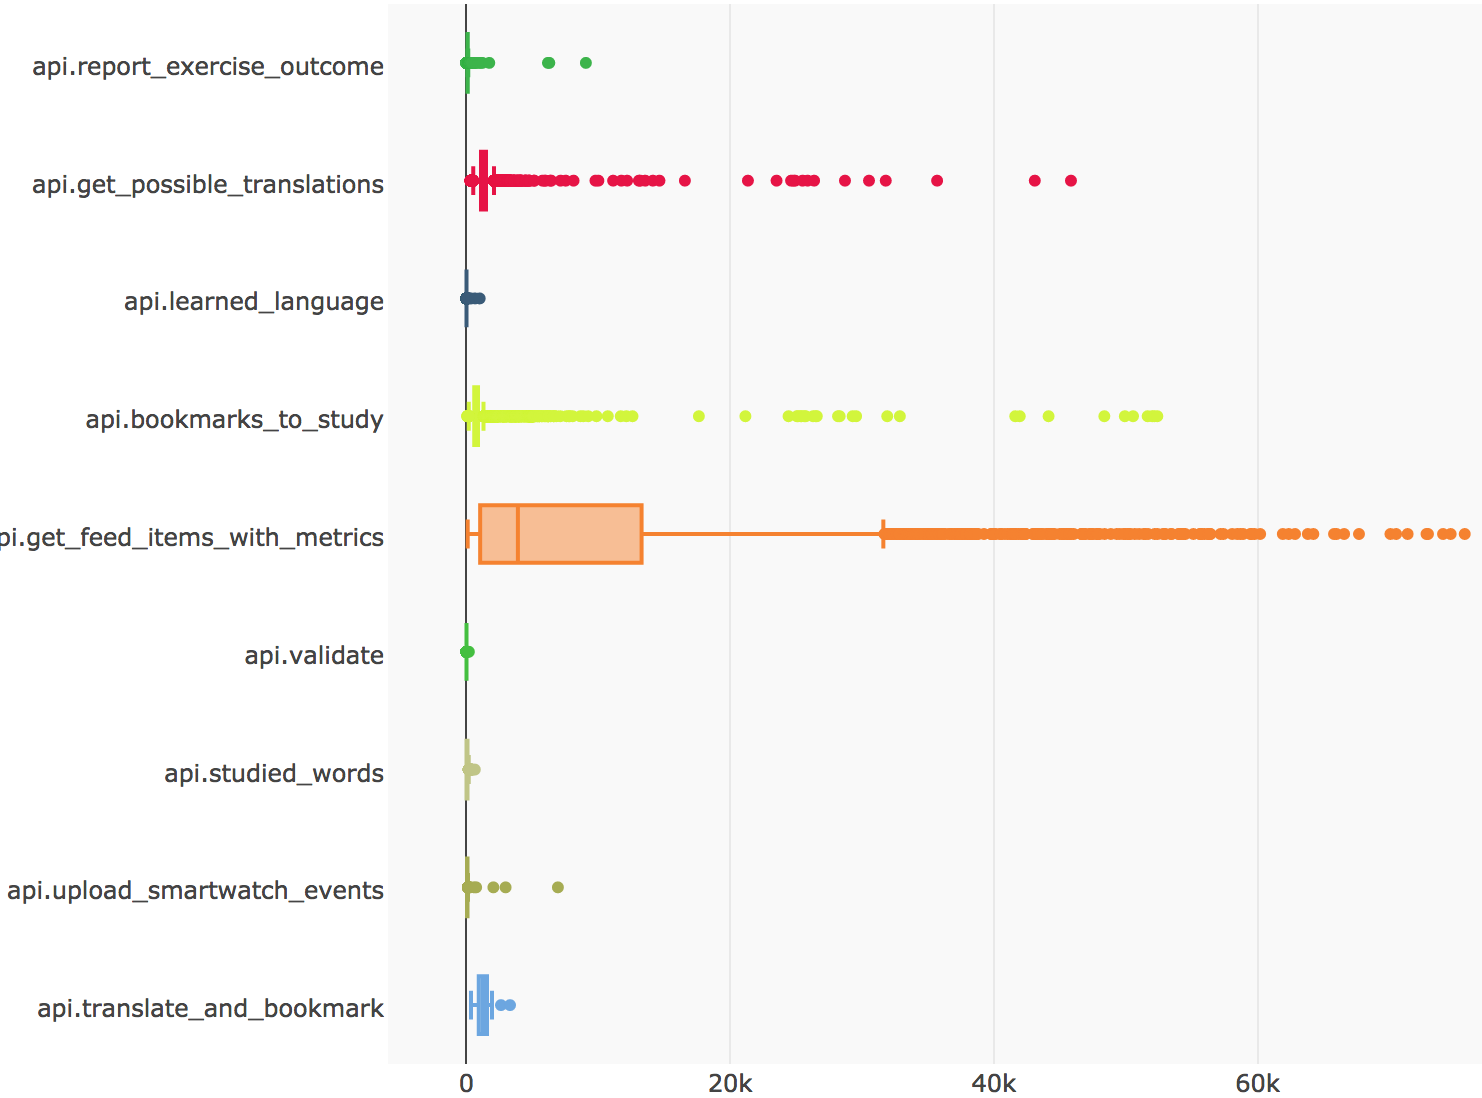
\includegraphics[width=0.95\linewidth]{endpoint_performance_}
 \caption{The response time (in ms) per monitored endpoint view allows for identifying performance variability and balancing issues}
 \label{fig:ep}
\end{figure}

The \perspective{API Performance} perspective is important for allocating optimization efforts. In our case study, after seeing this perspecgive, the API developers decided to rearchitect the system in order to improve the performance of \epTranslations and \epFeedItems. 

% However, in order to understand the problems of the two endpoints, a big component represents understanding the outliers: because they are many. \va{the last sentence does not parse} 







